\chapter{Threat Modelling}

Threat modelling is an act of security analysis which aids in discovering potential vulnerabilities in an application or a system before they become threats \citep{threat_model_intro}. This exercise is a crucial step in the Software Development Life Cycle (SDLC), as it helps detect the possible flaws in the system, and suitable mitigation can be applied. Similarly, threat modelling will also be conducted for this project, where an authentication server using OIDC protocol is operated in a cloud environment. The approach that this project will apply to threat modelling is based on Shostack's Four Question Framework \citep{shostack}. The questions focus on the project objectives, what could go wrong there, what mitigations could be applied, and whether it can be improved. Using Shostacks questions in conjunction with the OWASP threat modelling process, the application, using OpenID Connect in Cloud, can be analysed \citep{owasp_threat_model}. 


\section{Application Information}
To answer the first question about \textit{what are we working on}, this section will describe the application and the different dependencies that this application contains.
\begin{itemize}
    \item \textbf{Application Name:} Multi-tenant App
    \item \textbf{Application Version:} v1.0
    \item \textbf{Description:} This generic authentication and authorisation application utilises OpenID Connect protocols PKCE flow (See Figure \ref{fig:pkce_flow}) in a public cloud environment. This application will be based on multitenant capability, where the users cannot access each other's resources even though they share the same infrastructure and application. This is a general API which would provide the capabilities mentioned in Table \ref{table:threat_model_entry_points}.
  \end{itemize}

\subsection{Entry Points}
\begin{longtable}{|p{3cm}|p{4cm}|p{4cm}|p{4cm}|}
\caption{Threat modeling: Entry Points}
\label{table:threat_model_entry_points}
\hline
\rowcolor{grey!15}
\textbf{Entry Point} & \textbf{Description} & \textbf{Request Parameters} & \textbf{Response Data} \\
\hline
\endfirsthead
\hline
\rowcolor{grey!15}
\textbf{Entry Point} & \textbf{Description} & \textbf{Request Parameters} & \textbf{Response Data} \\
\hline
\endhead
\endfoot
\hline
\endlastfoot

/login & Entry point for user authentication.  & 
- client\_id: The client ID of the application \newline 
%- redirect\_uri: URI where the response will be sent \newline
- scope: Scopes for requested authentication (e.g., OpenID, email) \newline 
- response\_type: Indicates the desired authorization flow (e.g., code) & 
- The authorisation code is to be exchanged for tokens. \newline 
- Error in case of invalid request \\
\hline

/token & Entry point for exchanging authorization code for tokens (access token, ID token, refresh token). & 
- grant\_type: Must be "authorization\_code" \newline 
- code: Authorization code received from /login \newline
%- redirect\_uri: Must match the original redirect URI used in /login \newline 
- client\_id: The client ID of the application & 
- access\_token: Token for accessing protected resources \newline 
- id\_token: Token containing user identity information \newline 
- refresh\_token: Token for obtaining new access tokens \newline 
- Error in case of invalid request \\
\hline

/userinfo & Entry point to retrieve user information using access token. & 
- access\_token: Token obtained from /token endpoint & 
- id: Unique identifier of the user \newline 
- email: User's email address \newline 
- name: User's full name \newline 
- Error in case of invalid token or request \\
\hline

/logout & Entry point for logging out the user and invalidating tokens. & 
- post\_logout\_redirect\_uri: URI to redirect after successful logout & 
- Redirect to post\_logout\_redirect\_uri \newline 
- Error in case of invalid token or request \\
\hline

\end{longtable}
\section{Data Flow Diagram}
As a first step to identify what is the intention of the project, a data flow diagram (See Figure XX)

\begin{figure}[h!]
\centering
\caption{Data Flow Diagram Level 1 OIDC App}\label{fig:dfd_app}
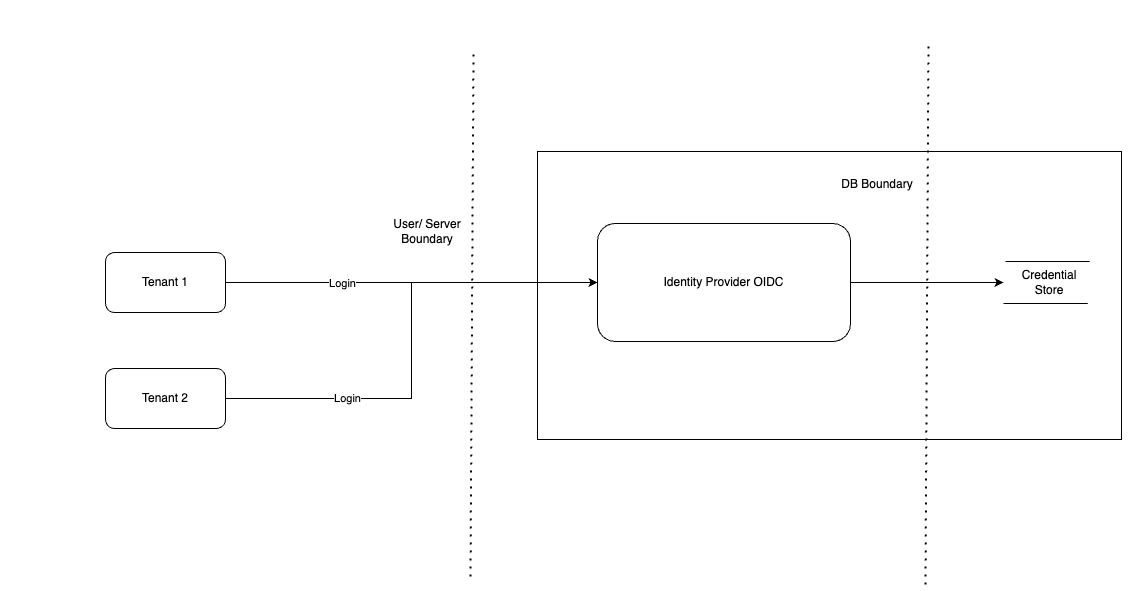
\includegraphics[width=\textwidth, height=320px]{pics/DFD_APP.png}
\end{figure}

\section{STRIDE Model}


\section{Mitigations}